\documentclass[a4paper,12pt,oneside]{book}
\usepackage[utf8]{inputenc}
\renewcommand{\chaptername}{Part}

\usepackage{rachwidgets}

\titleformat{\chapter}[display]
  {\bfseries\Large}
  {\filright\MakeUppercase{\chaptertitlename} \Huge\thechapter}
  {1ex}
  {\titlerule\vspace{1ex}\filleft}
  [\vspace{1ex}\titlerule]

\newcommand{\laClass}       {CS 250}
\newcommand{\laSemester}    {Spring 2018}
\newcommand{\laChapter}     {}
\newcommand{\laType}        {Project}
\newcommand{\laAssignment}  {1}
\newcommand{\laPoints}      {5}
\newcommand{\laTitle}       {Bag ADT}
\newcommand{\laStarterFiles}{Download from GitHub.}
\newcommand{\laTopics}      {Data structures, array implementations}
\setcounter{chapter}{0}
\setcounter{section}{1}
\addtocounter{section}{-1}
\newcounter{question}
\toggletrue{answerkey}
\togglefalse{answerkey}

\title{}
\author{Rachel Singh}
\date{\today}

\pagestyle{fancy}
\fancyhf{}

\lhead{\laClass, \laSemester}

\chead{}

\rhead{\laType\ \laAssignment: \laTitle\ \iftoggle{answerkey}{ KEY }{}}

\rfoot{\thepage\ of \pageref{LastPage}}

\lfoot{\scriptsize By Rachel Singh, last updated \today}

\renewcommand{\headrulewidth}{2pt}
\renewcommand{\footrulewidth}{1pt}

\begin{document}




\footnotesize
~\\ 
\textbf{\laType\ \laAssignment: \laTitle \tab } 
Homework projects should be worked on by each individual student.
Brainstorming and sketching out problems on paper or on a whiteboard
together are permitted, but \underline{do not} copy code from someone else
or allow your code to be copied. Students who commit or aid in plagiarism will
receive a 0\% on the assignment and be reported.

\hrulefill
\normalsize 

    \subsection*{Information}
    
        \paragraph{Topics:} \laTopics

        \paragraph{Turn in:}
            Turn in all source files - .cpp, .hpp, and/or .h files.
            \textbf{Do not turn in Visual Studio files}.

        \paragraph{Starter files:} \laStarterFiles

        \paragraph{Building and running:} If you are using Visual Studio,
            make sure to run \underline{with} debugging. (Don't run without debugging!)
            Using the debugger will help you find errors. \\
            To prevent a program exit, use this before \texttt{return 0;}
\begin{verbatim}
cin.ignore();
cin.get();
\end{verbatim}

        \paragraph{Tips:}
            \begin{itemize}
                \item   \underline{Always make sure it builds.}
                        Only add a few lines of code at a time and build
                        after each small change to ensure your program still builds.
                        
                \item   \underline{One feature at a time.}
                        Only implement one feature (or one function) at a time.
                        Make sure it builds, runs, and works as intended before
                        moving on to the next feature.
                        
                \item   \underline{Search for build errors.}
                        Chances are someone else has had the same build error before.
                        Copy the message into a search engine and look for information
                        on \textit{why} it occurs, and \textit{how} to resolve it.

                \item   \underline{Use debug tools,} such as breakpoints,
                        stack trace, and variable watch.
                
                \item   \underline{Don't implement everything in one go.}
                        Don't just try typing out all the code in one go
                        without building, running, and testing. It will be
                        much harder to debug if you've tried to program everything all at once.
            \end{itemize}

        \tableofcontents

    \newpage


    \chapter{About}

        For this first project, we will step through implementing
        a bag object with a static array. This project will be a bit
        hand-holdey, so you can get used to the tools and basics of
        coding in C++.

        You can also use Chapter 3 of the textbook for additional information
        on how to implement these functions.

        \chapter{Project setup}

        \section{Setting up an IDE}

            IDE stands for ``Integrated Development Environment''. An IDE
            is a program that contains the text editor for code, as well
            as some project management tools and debugging tools.

            We will step through how to create a project in both Visual Studio
            and in Code::Blocks. If you're working on your own computer,
            you can get a free version of Visual Studio Community Edition. If
            VS is too bulky or slow, or if you're not running Windows, then
            Code::Blocks is a good option as well.

            \paragraph{Visual Studio:}
                \texttt{https://www.visualstudio.com/vs/community/}

            \paragraph{Code::Blocks:}
                \texttt{http://codeblocks.org/downloads/26}

                Note: If installing for Windows, download the version that
                says ``mingw-setup.exe''.

        \newpage

        \section{Creating a project}

            \subsubsection{In Visual Studio}

                When you first open up Visual Studio, it will have a welcome page.
                You can select New Project from here, or from File $>$ New $>$ Project...

                \begin{figure}[h]
                    \centering
                    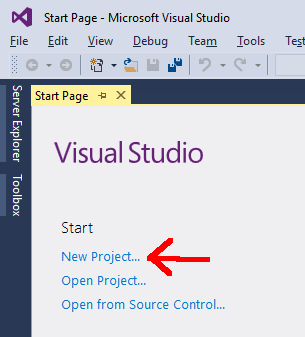
\includegraphics[width=5cm]{images-2018-01/vs-newproject.png}
                    %\caption{The ``New Project...'' button in Visual Studio}
                \end{figure}

                On the New Project dialog window, make sure to select Visual C++ on the left side,
                and then Empty Project in the middle pane.
                (Note: You might have to install additional files to use C++)

                Set the project Name and Location at the bottom.
                
                \begin{figure}[h]
                    \centering
                    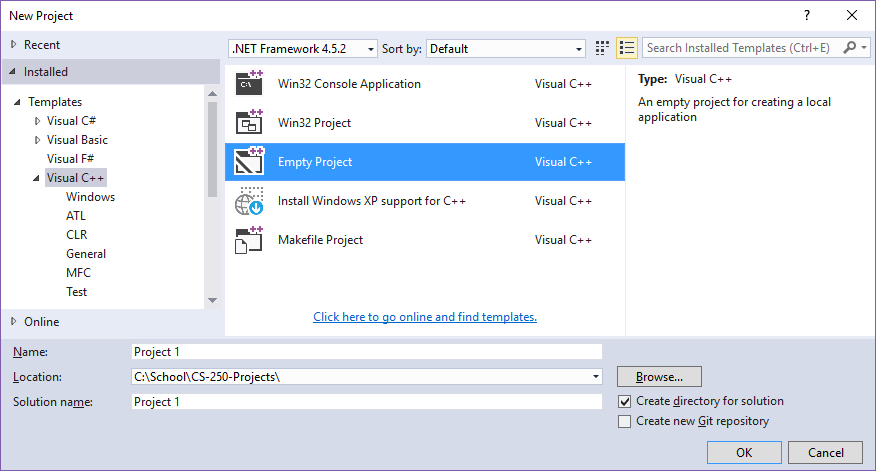
\includegraphics[width=14cm]{images-2018-01/vs-newproject2.png}
                    %\caption{Selecting ``Empty Project'' and setting Name and Location.}
                \end{figure}

                Afterwards, click on OK.

                The project is created, but will be empty and contain no source files.

                To add an empty file, In the Solution Explorer, right-click your project file and go to Add $>$ New Item...

                \begin{figure}[h]
                    \centering
                    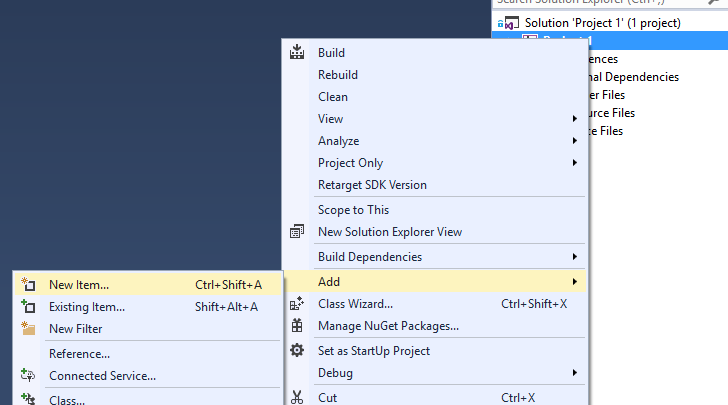
\includegraphics[width=12cm]{images-2018-01/vs-addnewitem.png}
                    %\caption{Selecting ``Empty Project'' and setting Name and Location.}
                \end{figure}

                If you're creating the file to store your main() function, select the C++ File.
                
                \begin{figure}[h]
                    \centering
                    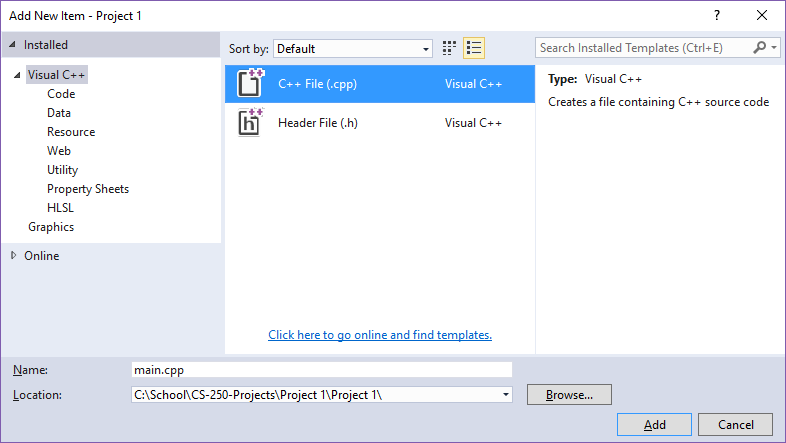
\includegraphics[width=14cm]{images-2018-01/vs-newcpp.png}
                    %\caption{Selecting ``Empty Project'' and setting Name and Location.}
                \end{figure}

                Give it a name, and click Add.

            \newpage

            \subsubsection{In Code::Blocks}

                When you first open up Code::Blocks, it will have a welcome page.
                You can select Create a new project from here, or from File $>$ New $>$ Project...
            
                \begin{figure}[h]
                    \centering
                    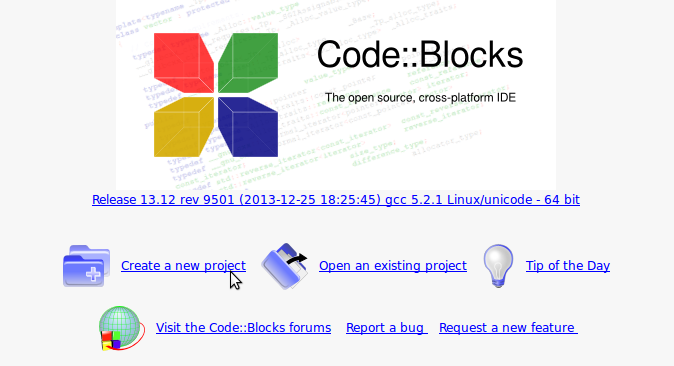
\includegraphics[width=12cm]{images-2018-01/codeblocks_newproject.png}
                \end{figure}

                On the New from template window that pops up, select Empty project and click Go.
            
                \begin{figure}[h]
                    \centering
                    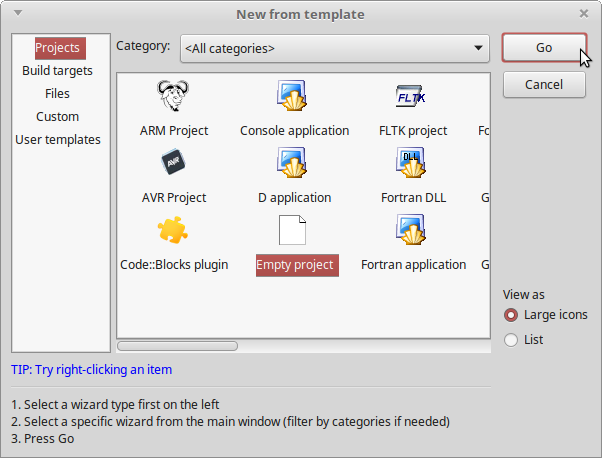
\includegraphics[width=10cm]{images-2018-01/codeblocks_emptyproject.png}
                \end{figure}

                \newpage

                On the next screen...
            
                \begin{figure}[h]
                    \centering
                    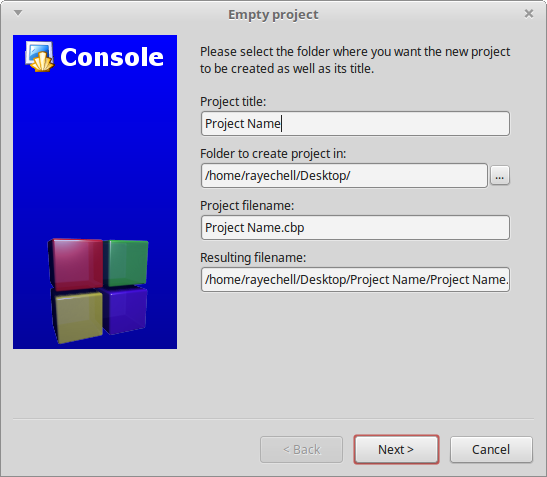
\includegraphics[width=10cm]{images-2018-01/codeblocks_newproject_dialog.png}
                \end{figure}

                first click ``...'' and select a directory where you want to store your project folder.

                After you have done so, give your project a title - a folder will be created for it automatically.

                Then click Next.

                \newpage

                The next window asks about Debug and Release options - leave these as the defaults and click Finish.
            
                \begin{figure}[h]
                    \centering
                    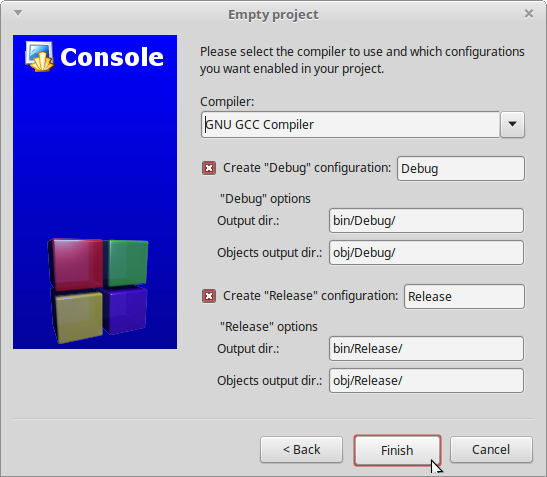
\includegraphics[width=10cm]{images-2018-01/codeblocks_debugrelease.png}
                \end{figure}

                The project will be empty. To add a new file, do the following:

                Go to File $>$ New $>$ Empty file.

                It will ask, ``Do you want to add this new file in the active project (has to be saved first)?''
                Click on ``yes'' and save your source file. Make sure the filename ends with ``.cpp''.
                Click ``Save'' once done making the file.
            
                \begin{figure}[h]
                    \centering
                    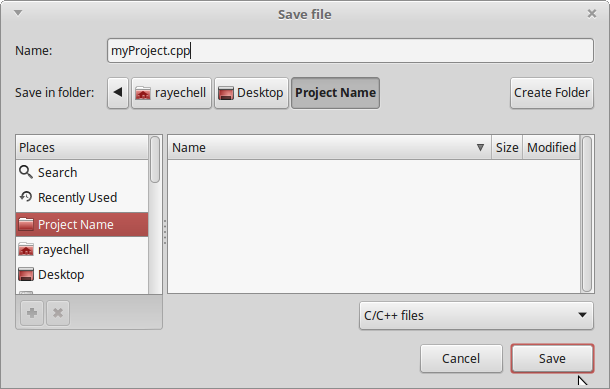
\includegraphics[width=10cm]{images-2018-01/codeblocks_newfile.png}
                \end{figure}

                Another window pops up asking about debug and release. Leave these both checked and click Ok.
            
                \begin{figure}[h]
                    \centering
                    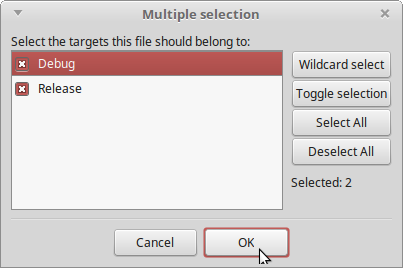
\includegraphics[width=10cm]{images-2018-01/codeblocks_debugagain.png}
                \end{figure}

        \section{Creating files}

            For this project, you will need to make two files: A .cpp file to store your program code,
            and a header file, ``Bag.hpp''. Your .cpp file can have any name, such as ``project1.cpp'',
            ``main.cpp'', etc.

            \begin{intro}{Why .hpp?}
                Many C++ programmers will name their header files with the .h extension, but some use
                .hpp. A common reason for this is if you're writing code FOR C++, not for C AND C++ together.
                Some libraries were written in C but can be used in both languages, while libraries
                written IN C++ and FOR C++ may opt to use ``.hpp'' as their header extensions.
            \end{intro}

        \newpage

        \section{Starter code}

            In your .cpp source file, let's start out with some basic code.
            Type out the following:

\begin{lstlisting}[style=code]
#include <iostream>
#include <string>
#include "Bag.hpp"

using namespace std;

int main()
{
    cout << "Hello, world!" << endl;

    // Don't let the program stop immediately
    cin.ignore();
    cin.get();

    return 0;
}
\end{lstlisting}

            \paragraph{Visual Studio:} To build and run in Visual Studio, click on the ``Local Windows Debugger'' button or hit F5.
        
            \begin{figure}[h]
                \centering
                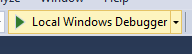
\includegraphics{images-2018-01/vs-play.png}
            \end{figure}

            It may ask if you want to build first before you run. Click on Yes -- You will always want to click on Yes here.

            If the build fails, it will ask if you still want to run - say NO. Otherwise, if the build was successful, it will run your program.

            \begin{error}{Always run with the debugger}
                In the past, you might have gone through the dropdown menu and
                started your program \textit{without} debugging so that the program
                wouldn't exit immediately. \textbf{DON'T DO THIS.}
                The debugger gives you invaluable tools for fidning errors and dealing
                with crashes.
            \end{error}

            ~\\
            \paragraph{Code::Blocks:} To build and run in Code::Blocks, click on the ``Build and run'' button, or hit F9.
            
            \begin{figure}[h]
                \centering
                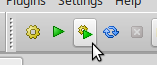
\includegraphics{images-2018-01/codeblocks_buildrun.png}
            \end{figure}

            Make sure the program builds and runs before continuing.

    \chapter{Creating the Bag class}

        For now, we will be working in the Bag.hpp file. First, we need
        to add the preprocessor directives to make sure no issues occur
        should the .hpp file be included from multiple source files.

\begin{figure}[h]
\begin{lstlisting}[style=code]
#ifndef _BAG_HPP
#define _BAG_HPP

#endif
\end{lstlisting}
\caption*{Bag.hpp}
\end{figure}

        The labels here, \texttt{\_BAG\_HPP}, are up to you,
        but they should be something unique enough to cut down on the
        likelihood that you'd have naming conflicts.

        Next, we will create the templated class declaration:

\begin{figure}[h]
\begin{lstlisting}[style=code]
template <typename T>
class Bag
{
private:
public:
};
\end{lstlisting}
\end{figure}

        Templates allow us to create container classes that can store
        \textit{any} data type. Instead of writing separate Bags for \texttt{int},
        \texttt{string}, \texttt{float}, etc. data types, we use the
        type-name \texttt{T} as a placeholder.

        \newpage

        \section{Variable and function declarations}

        The Bag class will have the following private member variables:

        \begin{center}
            \begin{tabular}{p{3cm} p{3cm} p{6cm}}
                \textbf{Name} & \textbf{Data type} & \textbf{Description}
                \\ \hline
                \texttt{m\_itemCount} & integer & Keeps track of the amount of items inserted in the array.
                \\ \\
                \texttt{ARRAY\_SIZE} & const integer & Keeps track of the size of the array.
            \end{tabular}
        \end{center}

        And it will have the following private member methods:
        
        \begin{center}
            \begin{tabular}{p{7cm} p{6cm}}
                \textbf{Function header} & \textbf{Description}
                \\ \hline
                \texttt{void ShiftRight( int atIndex )} & Moves everything \textit{atIndex} and afterwards to the right by 1 spot.
                \\ \\
                \texttt{void ShiftLeft( int atIndex )} & Moves everything after \textit{atIndex} to the left by 1 spot.
            \end{tabular}
        \end{center}

        And the following public member methods:
        
        \begin{center}
            \begin{tabular}{p{7cm} p{6cm}}
                \textbf{Function header} & \textbf{Description}
                \\ \hline
                \texttt{Bag()}
                    & The constructor, which initializes member variables.
                \\ \\
                \texttt{~Bag()}
                    & The destructor.
                \\ \\
                \texttt{int Size() const}
                    & Returns the amount of items store in the array.
                \\ \\
                \texttt{bool IsEmpty() const}
                    & Returns whether the array is empty.
                \\ \\
                \texttt{bool IsFull() const}
                    & Returns whether the array is full.
                \\ \\
                \texttt{bool Push( const T\& newItem )}
                    & Adds a new item to the end of the sequence of items.
                \\ \\
                \texttt{bool Pop()}
                    & Removes the last item in the sequence.
            \end{tabular}
        \end{center}
        
        \begin{center}
            \begin{tabular}{p{7cm} p{6cm}}
                \textbf{Function header} & \textbf{Description}
                \\ \hline
                \texttt{void Clear()}
                    & Clears out the list.
                \\ \\
                \texttt{int GetCountOf( const T\& item ) const}
                    & Returns the amount of instances of the given item in the array.
                \\ \\
                \texttt{bool Contains( const T\& item ) const}
                    & Returns whether the item is contained in the array.
                \\ \\
                \texttt{bool Remove( const T\& item )}
                    & Remove all items that match.
                \\ \\
                \texttt{bool Remove( int atIndex )}
                    & Remove the item at a specific index.
                \\ \\
                \texttt{bool Insert( int atIndex, const T\& item )}
                    & Insert an item in the middle of other items.
                \\ \\
                \texttt{T\& Get( int atIndex )}
                    & Get an item in the array at a specific index
                \\ \\
                \texttt{T\& GetFront()}
                    & Get the first item in the array.
                \\ \\
                \texttt{T\& GetBack()}
                    & Get the last item in the array.
            \end{tabular}
        \end{center}

        We will implement each of these one-at-a-time, and write tests
        to check the functionality.

        \section{Constructor and destuctor}

        \section{Implementing Push}

        \section{Implementing Size and testing}

        \section{Implementing IsEmpty and IsFull and testing}

        \section{Implementing Get, GetFront, and GetBack and testing}

        \section{Implementing Contains and testing}

        \section{Implementing GetCountOf and testing}

        \section{Implementing Clear and testing}

        \section{Implementing Insert and ShiftRight and testing}

        \section{Implementing Pop and testing}

        \section{Implementing Remove and ShiftLeft and testing}
                
    \newpage

    \chapter{Example output}

    \chapter{Grading breakdown}



\end{document}

